\documentclass[10pt]{article}
\usepackage{amsmath}
\usepackage{amsfonts}
\usepackage{amssymb}
\usepackage{graphicx}
\usepackage{hyperref}

\author{Joshua Horswill}
\title{Firmware Block Implementation for the Proto-DUNEII Hit Finding Architecture with the HLS Tool - First Semester Report}

\begin{document}
\maketitle

\begin{abstract}
	The Deep Underground Neutrino Experiment (DUNE) is a large-scale international project being developed at CERN and will operate within North America. It will consist of two underground neutrino detectors placed within an intense neutrino beam fired from Fermilab, the furthest of which will be 1300 kilometres from the source, in the Sanford Underground Research Facility (SURF). The main objectives of the experiment include answering fundamental questions about the origin of matter, namely certain properties of leptonic CP violation. There are also aims to investigate the unification of forces through the analysis of proton decay, and the formation of black holes through supernova neutrino detection\cite{deep_underground_neutrino_experiment_2020}. This report focusses on the TPG cores within the front-end electronics of the detectors, specifically the hit finder architecture that processes optical data generated from argon scintillation within the time projection chambers, as a result of neutrino-nucleon interactions. The focus of  discussion will be on the replacement of existing firmware algorithms written for the detector's Field-Programmable Gate Arrays (FPGAs) with designs synthesised via Vivado High Level Synthesis (HLS) from C++ code. The purpose of this is to test the efficiency and convenience of the block design process when compared to writing firmware from scratch in VHDL.
\end{abstract}

\newpage
\tableofcontents

\newpage

\section{Introduction}

\subsection{DUNE Experiment Background and Goals}
The DUNE experiment is an amalgamation of many neutrino-physics communities, centred around an opportunity provided by the large investment of the U.S. Department of Energy. This will contribute to a large expansion of the underground experimental architecture of the SURF facility, as well as a megawatt neutrino-beam facility 1300km across North America at Fermilab. This investigation will be groundbreaking for several areas of physics, including neutrino oscillation studies, searches for proton decay, and for neutrino based astrophysics (black hole and supernova burst phenomena).

Analysing the properties of neutrinos has led to evidence for physics beyond the Standard Model (SM). Oscillations of neutrino flavour i.e. a neutrino's ability to transform their flavour after moving through space, is a well established concept. Several conclusions can be made from this, including the fact that neutrinos have mass, although unexpectedly small. The sum of the three neutrino mass eigenstates must be less than one million of an electron mass eigenstate \cite{Mertens_2016, cooper2016masses}. The origin of these small neutrino masses and their oscillations is still not confirmed however, and is up for debate. Finding the explanation will require access to more precision and detail in the available experimental data. DUNE exists to carry out an investigation of neutrino oscillations to test `Lepton sector CP Violation' (LCPV) as well as the ordering of the neutrino masses and the three-neutrino paradigm, in which the quantum mechanical mixing of the three neutrino mass eigenstates produces the three known neutrino flavour states \cite{acciarri2016longbaseline}.

CPV is well established in Quantum Chromodynamics (QCD), allowed by the complex-natured Cabibbo-Kobayashi-Mashawa (CKM) matrix\footnote{Used to contain the information on the strength of the flavour-changing weak interaction \cite{kobayashi1973cp}.}\cite{kobayashi1973cp}. Therefore one would expect to discover an entirely analagous mechanism to arise in the lepton sector of the standard model (SM), leading to LCPV. One of the collaboration's goals is to determine the rates at which neutrino CP violation occurs within the lepton sector. Another hypothesis proposes that there is a connection between low-energy neutrino physics and leptogenesis \cite{Di_Bari_2012}, which could provide insight into the scenario that led to the baryon asymmetry of the universe. These questions can only be answered by constructing suitable detector equipment; the next section will explore the features of ProtoDUNE's detector's front-end electronics and Data Acquisition (DAQ) system. This will feed into the following section that discusses the HLS firmware blocks that could instruct the front-end FPGA-based data processors.

\subsection{ProtoDUNE DAQ System}\label{section:overview}

DAQ architecture can be split into two parts: the front-end and the back-end. The front-end is comprised of electronics that acquire the data stream from readout-electronics from the TPC detector, so it can process and deliver it to the back-end: an offline storing, event-reconstruction computation farm. The focus of this report will be on the front-end, including the detection modules and the interface to the detector electronics.

There are several main factors that influence the design of the DUNE DAQ system. One of which is the hardware and maintenance cost per input channel, which is related to the technology life-cycle of each component. This contributes to the need for long-lasting essential parts such as the Xilinx FPGAs and network components. DUNE is set to run for approximately 20 years; the reliability and maintenance of the detector components is more important when compared to other large-scale projects. The power consumption of the detector modules also requires consideration due to cooling contingencies and the variance in running costs. Another motive for the design would be modularity of the hardware and firmware blocks, so that one change in a sub-module would not affect the rest. This emphasis on customisability carries over to the HLS design process, talked about in section \ref{HLS_section}. With this in mind, R\&D and fast firmware modifications can be a quick and efficient process. If the design tools are more abstract and are rooted in commonly used languages such as C++, this will appeal to the vast majority of the users (physicists) \cite{abi_barr_martin-albo_azfar_2017}.

\subsubsection{Single and Dual Phase LAr TPCs}

The use of Time Projection Chamber modules of Liquid Argon (LAr TPCs) is a matured and popular technique used by several short-baseline\footnote{The baseline of a neutrino experiment refers to the scale of the beam travel distance. DUNE is `long baseline' as the detector is positioned across the continent from the beam source.} neutrino experiments. They are popular for several reasons:

\begin{itemize}
	\item Argon is a noble element which has vanishing electronegativity\footnote{Low tendency to attract a shared pair of electrons in an atomic bond.} which means that electrons produced by ionizing radiation will not be absorbed as they drift towards the detector.
	\item  Liquid Argon is inexpensive yet very dense, increasing the likelihood of a particle interacting by 1000 times when compared to Nygren's TPC design \cite{rubbia1977liquid}. This is important because the cross section for neutrino-nucleon interactions is very small.
	\item A neutrino-nucleon interaction causes the Argon to scintillate; a secondary energetic charged particle is generated and travels through the liquid, which causes the release of scintillation photons, the number of which is proportional to the energy deposited by the passing particle \cite{adams2018rejecting}. This contributes to the reconstruction of the event. 
	
\end{itemize}

\begin{figure}
	\centering
	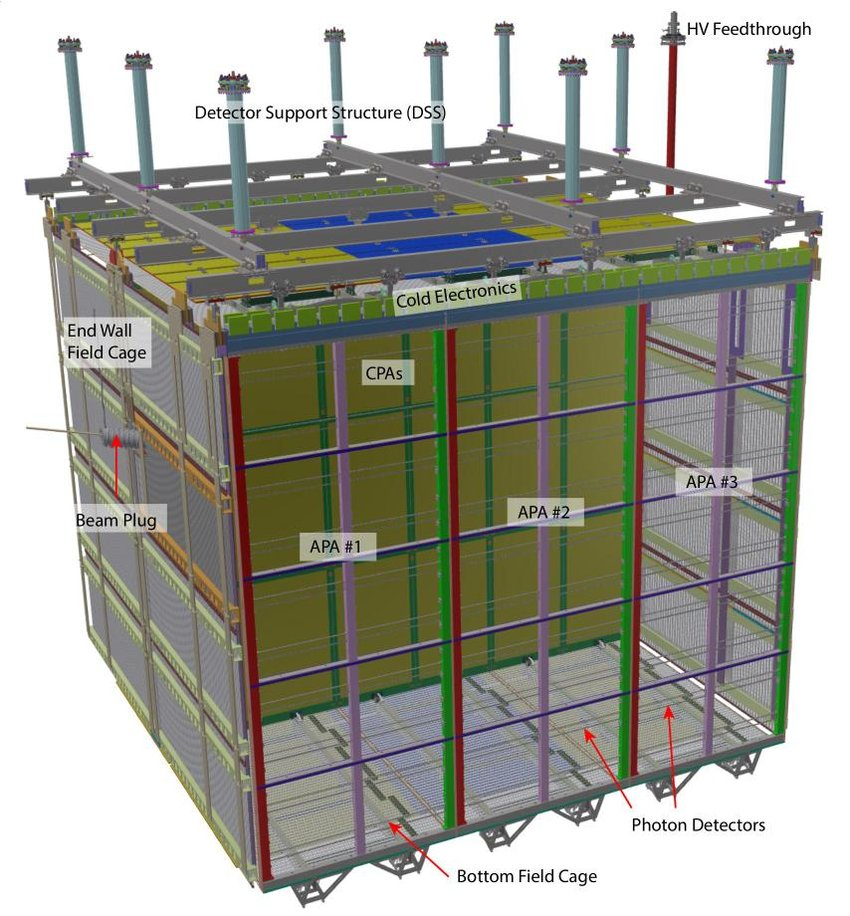
\includegraphics[width=0.7\linewidth]{figures/The-major-components-of-the-ProtoDUNE-SP-TPC}
	\caption[ProtoDUNE-SP]{Diagram of the ProtoDUNE single-phase LAr TPC module. This contains two drift volumes, separated by a central cathode plane that is flanked by two anode planes, connected to a field cage that surrounds the entire module. Each anode plane is made of three Anode Plane Assemblies (APAs). These connect and send data to the front-end electronics being discussed in this report \cite{dune_sp_collab}.}
	\label{fig:the-major-components-of-the-protodune-sp-tpc}
\end{figure}


 There exists both single and dual-phase versions of these LAr TPC modules. Inside single-phase liquid argon detectors, such as the structure featured in figure \ref{fig:the-major-components-of-the-protodune-sp-tpc}, the interactions are readout by wires immersed in the liquid and do not require the amplification of the ionized electron charge. The charge is localised using alternative induction and collection wire planes with different orientations. This was tested by ProtonDune-SP at CERN \cite{dune_sp_collab}.
 
 The dual phase detectors rely on the amplification of ionisation charges in the ultra-pure cold-argon vapour layer above the liquid, obtaining low-energy detection thresholds with high signal-to-noise ratio over drift distances exceeding 10m. In dual-phase LAr TPCs, ionisation charges produced by neutrino interactions drift vertically towards the liquid-vapour boundary where they are extracted into the `gas phase', amplified by components named Large Electron Multipliers (LEMs), and collected by segmented anodes; the electron extraction, amplification and collection are performed inside a $3 \times 1 \ \text{m}^2$ frame called the charge readout plane (CRP). Bear in mind the dimensions of the detector prototype are $3 \times 1 \times 1 \ \text{m}^3$. 
 Five photo-multiplier tubes are mounted underneath the TPC drift cage. They detect the Argon (prompt S1) scintillation photons formed from passing charged particles, as well as the (proportional S2) secondary scintillation light from the electroluminescence of the electrons extracted in the argon vapour. S1 is at least several orders of magnitude higher in detection amplitude than S2 in a tested TPC \cite{aimard20184}.
 
 The 10 kilo-tonne dual-phase liquid argon TPC is one of the main detector options considered for DUNE. LAr TPC's offer unprecedented 3D imaging capabilities and the functionality of a homogeneous calorimeter. High-resolution imaging is the key to efficient background noise rejection.

\subsection{FELIX}

The LAr TPC modules used in the ProtoDUNE II design contain 150 anode plane assemblies (APA's) with 2560 wires per APA. There are 10 fibres/data streams in the APA, each with 256 wires - hence the total of 2560. The Front End LInk eXchange (FELIX) system is used to receive the data from the APAs, and was first developed within the ATLAS collaboration. Within this system contains the focus of this project: the Trigger Primitive Generation (TPG) core, which will be discussed in more detail later.

FELIX is a PCIe-based\footnote{High speed connection ports used in motherboards to connect GPUs, SSD's, wifi chips and more} high-throughput approach that was originally developed for interfacing front-end and trigger electronics in the ATLAS Upgrade framework. It was implemented due to the ATLAS phase-I upgrade requiring a Trigger and Data Acquisition (TDAQ) system able to trigger and record data from up to three times the nominal LHC instantaneous luminosity. The FELIX system provides the infrastructure to achieve this in a scalable, detector agnostic and easily upgradeable way. The interface enables the reduction of custom electronics in favour of software running on commercial servers. It is a PC-based networking gateway with the FPGA mounted on PCIe Gen3 cards \cite{borga2019felix}. In ProtoDUNE II, FELIX interfaces with and manipulates the data from the APA, during which time it is fed through the internal hit-finder TPG core.

The readout window per neutrino event is between 3-5.5 ms for a 2.25 ms drift time. The FELIX architecture that handles this influx of events consists of 10 MGT modules, the function of which is to process the APA data stream into computational bits, which are then fed into 10 Hit Finders (HF), as seen in figure \ref{fig:fearch}. The hits are produced by processing the incoming ADC (Analog-to-Digital Converted) samples in parallel. The MGT output enters the HFs via the data router, which receives multiple-channel, single clock-tick packets. The packets initially exist in a format containing a given sample for all channels, and when processed by the data router are converted into a format subsisting of all the samples for a given channel i.e. multiple clock ticks of data. The formatted output is then transferred into 10 sets of 4 TPG block processors; one set for each MGT output. These are multiplexed\footnote{Combined into a singular signal output} by the arbitrator into the Central Router (CR) interface \cite{abi_barr_martin-albo_azfar_2017, adams2020protodune} as seen in figure \ref{fig:hfprocessor}.

\begin{figure}[h]
	\centering
	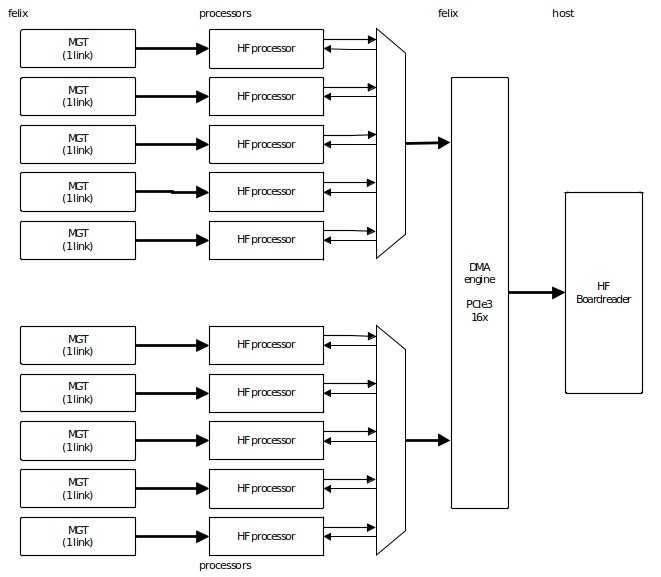
\includegraphics[width=0.7\linewidth]{figures/FE_arch}
	\caption{Overview of the Felix architecture in ProtoDUNE \cite{manolopoulos_2020}}
	\label{fig:fearch}
\end{figure}

\begin{figure}
	\centering
	\makebox[\textwidth][c]{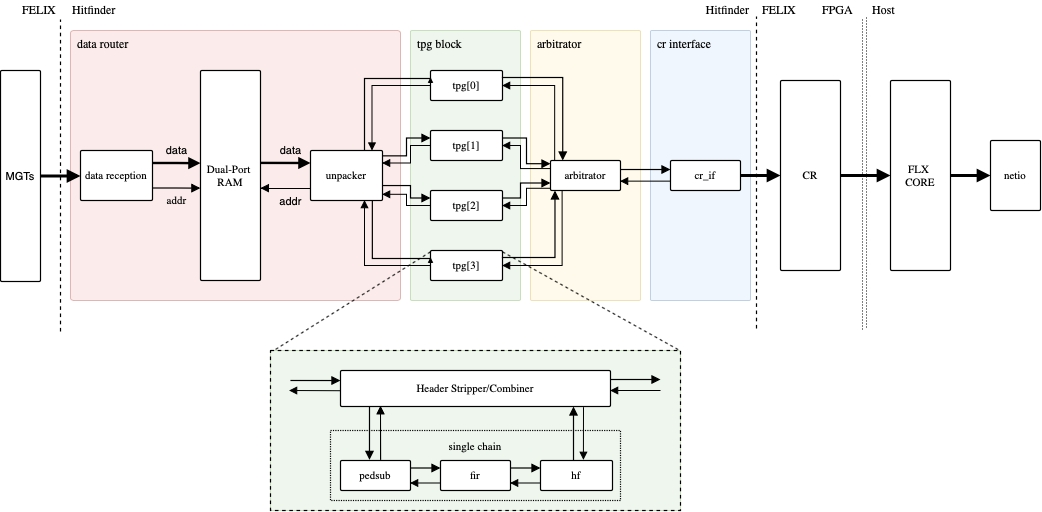
\includegraphics[width=1.6\linewidth]{figures/HF_processor}}
	\caption{Hit Finder Firmware Architecture \cite{manolopoulos_2020}.}
	\label{fig:hfprocessor}
\end{figure}

\subsection{The TPG Core}\label{tpgcoresec}

Each TPG unit processes the data from 64 APA wires, and so there are 4 of them for each core\footnote{$4\times 64 = 256$, the number of wires in a fiber; ten fibers summed over ten MGTs accounts for all wires within the APA (2560)}.
The TPG data consists of a header and payload. The header determines the source wire, the time stamp, and the origin of the data. The payload is 64 bits of ADC sample data for hit finding. There is an AXI4-stream protocol for unpacking and reordering of data in the TPG block, featuring 4 general signals for various instructions in each component:
	
	\begin{enumerate}
		\item tvalid denotes if the bus data is valid for processing
		\item tuser is a flag that denotes the end of a packet frame
		\item tlast indicates the end of a packet
		\item tready is used to apply back-pressure if the processing units ahead cannot process the data fast enough (all throughput is frozen).
	\end{enumerate}

Within the TPG core is a mechanism that strips the packet header; the Header Stripper/Combiner (HSC), featured in figure \ref{fig:hsc}. The header is sent to the output of the block. Meanwhile, the remaining 64 ADC samples and their associated AXI4 signals are processed by the PedSub (pedestal subtraction), FIR (finite impulse response), and HF sub-blocks in the chain. The data router is then signalled to send the next packet. The objective of this report is to redesign the firmware algorithms for the TPG sub-blocks in Xilinx's Vivado HLS software suite, to compare the performance and resource usage to the existing firmware written by VHDL engineers. Section \ref{HLS_section} goes into more detail on this matter.

\begin{figure}
	\centering
	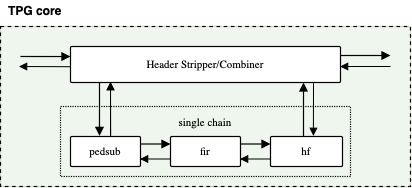
\includegraphics[width=0.7\linewidth]{figures/HSC}
	\caption{Focus on the HSC and the sub-block chain \cite{manolopoulos_2020}.}
	\label{fig:hsc}
\end{figure}

\section{HLS}\label{HLS_section}

\subsection{Background}
High-level synthesis (HLS) is an automated design process that interprets an algorithmic description of a desired behavior and creates digital hardware that implements that behavior. It was initially designed to increase the levels of abstraction of design methodologies, forced by the growing capabilities of silicon technology and the increasing complexity of their applications. Beginning in the 1950s, assembly languages were introduced and gradually evolved to high level languages with improved compilation techniques, obeying the intuitive rules of grammar, syntax and semantics. Gate-level simulations appeared in the 1970s, and in the 1980s progress led to Hardware Description Languages (HDLs)  i.e. languages that describe the structure and behaviour of electronic circuits, and more commonly digital logic circuits \cite{coussy2009introduction}. HDLs look like programming languages such as C, but the main difference is that HDLs include the notion of clock timing. The most commonly-used languages are Verilog and VHDL, the latter of which is used in the DUNE firmware framework. HLS allows for a connection between software languages and hardware implementation, in this case of section \ref{pedsubalg} via VHDL firmware. 

Synthesis begins with a high-level specification of the problem, where behavior is generally decoupled from low-level circuit mechanics such as clock-level timing. Early HLS explored a variety of input specification languages, although recent research and commercial applications generally accept synthesizable subsets of ANSI C, C++, SystemC and MATLAB. C++ was used to design the algorithms featured in section \ref{pedsubalg}. This input source code is analysed, architecturally constrained, and scheduled to transcompile into a register-transfer level (RTL) design in a chosen HDL, which is in turn commonly synthesized to the gate level by the use of a logic synthesis tool \cite{vivado_design_suite_user_guide_2018}.

RTL is a design abstraction which models a synchronous digital circuit in terms of the signal flow between registers and the logic operations being performed on said signals \cite{vahid2010digital}. Hardware registers are circuits composed of flip flops (a sub circuit that has two stable states used to store state information; a basic storage element in sequential logic). They have the ability to read or write multiple bits at a time and can use an address to select a particular register, used as an interface between the software and the computer peripherals \cite{bose1996hardware}. RTL allows for circuitry simulation and digital analysis, and is used in HDLs to create high-level representations of a circuit, from which lower-level representations and ultimately actual wiring can be derived. RTL clock cycle data is given in Vivado HLS performance estimate data, as it can read how long a certain block, loop or function in the code took to complete; this is called the latency. Latency is a crucially important concept in RTL design, as it can make the difference between a system struggling with logic timing issues and a working synchronised circuit. Before the firmware block in question can be discussed, the design flow within Xilinx's Vivado HLS development software will be explained to provide context for the algorithm design.


\subsection{Vivado HLS Design Flow}
\label{section:HLS_DF}

The design flow when approaching the synthesis of a C algorithm is as follows:


\begin{enumerate}
	\item Compile, execute (simulate), and debug the C algorithm.
	
	This involves validating that the C program correctly implements the required processes. In order for this to occur, there must be a test bench written in C that includes the top-level function called within a simulation script, tasked with recreating the conditions of the implemented firmware, hosted within \texttt{main()}. This typically takes more time to design than the function to be synthesized.
	
	\item Synthesize the C algorithm into an RTL implementation, optionally employing user optimization directives that are further explained in section \ref{direct}.
	
	This allocates hardware resources such as BRAMS, buses, look up tables (LUTs), digital signal processors (DSPs) and registers. Each operation is scheduled to a certain clock cycle and bound to a functional unit within the board. Variables are bound to storage elements, and the RTL architecture is eventually generated\cite{vahid2010digital}.
	
	\item Generate comprehensive reports and analyze the design.
	
	After C synthesis, output files are stored in a directory which contains folders for each RTL output format, and a report folder. The report folder contains files reporting on the performance and design corresponding to the top-level function (the function to be synthesized) and each individual subfunction. The analysis tab allows for cycle-by-cycle insight into the timing of logic operations and the FPGA resource consumption that they require. This is the best opportunity to analyse the effect of applied function directives and \texttt{pragma} commands within the code.
	
	\item Verify the RTL implementation using a pushbutton flow.
	
	 This is a post-synthesis validation process that compares the synthesised RTL and C programs to see if they generate the same output; this is called RTL cosimulation.
	
	\item Package the RTL implementation into a selection of IP formats.
	
	This generates the verified VHDL script that can be synthesized in the Vivado project manager into an implementable design. Before this can occur, a wrapper is written to connect the IP block's I/O ports to the previous and following blocks, ensuring signals are being properly read and written. This is especially important for the AXI4 system discussed in section \ref{tpgcoresec}, as all signals must enter and leave the block to validate and manage the incoming and outgoing data samples. This can be tested in Questasim\footnote{Software dedicated to simulating HDLs. This is typically used in collaboration with the Vivado project manager environment.} to provide a waveform analysis of every port and internal signal involved. This is an important verification step in the design process, as the performance of an algorithm within the HLS environment can be vastly different to a VHDL simulation \cite{vivado_design_suite_user_guide_2018}.
\end{enumerate}

When writing HLS source code, there is punishment for using modern modules and storage entities; a simplified, classical style is most easily synthesized. Another constraint when establishing the desired behaviour for synthesis is that the top function must be written like an electronic circuit block, with an increased number of input and output function arguments when compared to a standard C program, so that post-synthesis, after arguments have been converted to RTL ports, there is ample interface for the wrapper to work with. Arrays must be pre-allocated memory, with a pre-determined number of elements (ruling out C++ vectors). The performance of the logic operations come into question when contrained by a certain latency in order for the block to operate as required. The clock frequency must simultaneously stay below $1/f_{target}$, which in the case of this report target frequency $f_{target} = 250$ MHz, meaning the clock duration must stay below 4ns. However, it must tick for long enough so that the block operations can occur within the desired latency. Performance comes at a trade to resource cost, as pipelining (parallelizing and rearranging operation initialisation to decrease latency) employs more FPGA elements, which are a finite resource. One way to reduce this cost is to assign accurate bit-widths to variables. Using standard C data types for hardware design results in unnecessary resource usage. Operations can use more LUTs and registers than needed for the required accuracy, causing delays that may exceed a given clock cycle, increasing the overall latency. Smaller bit widths (e.g using 17 bit data types for 17 bit multiplication rather than the standard C 32 bit data type) result in hardware operators which are smaller and faster. More logic can then fit in the FPGA and can operate at a higher clock frequency. The next section will discuss the management of performance and area when choosing HLS design guidances.

\subsubsection{Optimisations and Analysis}\label{direct}

Directives act as low-level guidance for the HLS tool, influencing the types of hardware used and the methods of implementing the source code operations. An example of this is a directive splitting an array construct into multiple RAM blocks to improve signal bandwidth, at the cost of increased resources \cite{lo2016model}. Different optimization directives can be applied before C synthesis:

\begin{itemize}
	\item Instruct a code task to execute in a pipeline, allowing the next execution of a task to begin before the current one finishes
	\item Specify a latency for the completion of functions and loops (one of the reasons for this is to match the FPGA clock frequency).
	\item Specify a limit to the resources used
	\item Select the I/O protocol to make sure the final design can be connected to other hardware blocks with the same I/O protocol.
\end{itemize}

There are several viable ways to achieve an optimal directive configuration for the purposes of the user, but the best way to see the effect of adding directives in the Vivado HLS tool is by analysing the cycle-by-cycle display of operations within the synthesis reports. We can analyse the performance estimates which involve a number of aspects, the first of which is clock timing; the fastest achievable clock frequency before the block ceases to function. This must meet the target so as to synchronise with the surrounding firmware blocks. The latency and initiation interval\footnote{The number of clock cycles before new inputs are processed.} (II) must be reviewed, since the internal operations of the block must have enough time to complete before the next input is processed. Without any pipeline directives, the latency defaults to one clock cycle less than the II so that this can be achieved. Finally, the utilization estimates are key to making the trade-off between latency and FPGA area, be it LUTs, FFs, DSP48s or single and dual-port BRAMS. Now that a sufficient introduction into the design process has been given, the next section will explore the key work outlined in this report: the HLS firmware algorithm design for the first sub block in the HSC (discussed in section \ref{tpgcoresec}).

%As well as performance and resource directives, there are instructions related to the block interface. There are three types of ports in the RTL design created by Vivado HLS:

%\begin{enumerate}
%	\item Clock and Reset ports: ap\_clk, ap\_rst
	
%	These respectively connect to the clock tick port and the full block reset port of the wrapper, to synchronise with the firmware network.
	
%	\item Block level interface protocols: ap\_start, ap\_done, ap\_ready and ap\_idle.
	
%	These are the signals that control the block independently of any port-level I/O protocols. ap\_start dictates when the block can start processing data, ap\_ready dictates whether it can accept new inputs, ap\_idle asserts low when the block is operating, and when the function completes ap\_done is asserted.
	
%	\item Port level interface protocols: created for each argument in the top-level function and the function return.
	
%	The I/O protocol depends on the type of C argument and on the switch default option. Port level IO protocols sequence the data in and out of the block once operation has been started by the above protocols. If there is no I/O protocol associated with the block output port, it is difficult to know when to read the data. Therefore it is always a good idea to use one on an output.
%\end{enumerate}

\section{Pedestal Subtraction Algorithm}\label{pedsubalg}

The pedestal subtraction algorithm is the first sub-block in the TPG core, fed by 64 sample words\footnote{One `packet' of samples.} from the Header-Stripper/Combiner, shown in figure \ref{fig:hsc}. The first 6 words (16 bit data types) are stripped from the incoming samples and sent to the \texttt{pedsub} block, where the `background noise' of the ADC values is removed. The algorithm is implemented as follows:

\begin{itemize}
	\item Each sample within the packet is scanned, subtracting the pedestal from each ADC value and adjusting the pedestal and accumulator variables according to the size of each ADC value. The firmware runs a AXI4 interface between blocks, which operates through a series of boolean signals mentioned in section \ref{section:overview}. \texttt{tkeep} and \texttt{treset} are two important signals that have not  been mentioned previously, the former of which goes high when the incoming data should be processed, and the latter when the entire process must be reset and restarted. The algorithm only runs when \texttt{tready} is low and \texttt{tvalid} and \texttt{tkeep} are high. \texttt{tlast} and \texttt{tuser} go high at the end of a packet. \texttt{treset} goes high when an error in the FELIX interface occurs.
	\item The user inputs an estimate of the median background value to subtract from the first few samples, as a temporary buffer before the pedestal value is changed by the algorithm.
	\item The algorithm also starts with an associated accumulator variable, initially equal to zero, that directly changes the pedestal value once it reaches $\pm10$. How does this accumulator variable change?
	\item The accumulator changes by $\pm1$ depending on the boolean (\texttt{ADCvalue} $>$ \texttt{pedestal}). If this boolean is true, the accumulator increases by one, and false means a decrease by one.
	\item The next condition is: if before a scan the accumulator is $+10$, the pedestal increases by one, and the accumulator is reset to zero. Then the next ADC value is subtracted by this new increased pedestal. The opposite is the case for an accumulator of $-10$; the pedestal decreases by one and the accumulator resets.
	\item At the end of each packet, the current value for the channel is stored and then retrieved from a state save/restore mechanism, for the next packet entering the channel.
\end{itemize} 

Eventually, with a large enough flux of packets, one would obtain a pedestal value appropriate for that input channel, giving more useful ADC values.

\subsection{Pedestal Subtraction Testbench}

The testbench of any design is one of the most important parts of any HLS project, and usually requires more time to complete than the source algorithm. The main purpose of the testbench is to validate the design when editing the top function so that it can C-simulate within the HLS compiler, synthesize and RTL/cosimulate to then be exported into an IP block. See section \ref{section:HLS_DF} for more detail on the firmware design flow.

The first testbench design generated an array of random ADC integer values within a reasonable range, and found the ideal pedestal value for that range. Subsequently, the testbench function scanned those ADC values with the subtraction algorithm and validated that the pedestal value converged to the expected value, or was equal to that value after a certain number of packets. This was acceptable to test the first iteration but it did not validate the adjusted ADC values output from the algorithm.

The output from a VHDL implementation of the \texttt{pedsub} algorithm was used to compare the output data of the HLS algorithm from one wave of packets travelling through 64 channels. This included a reading of the AXI4 signals, and a contingency for random raises of treset and tready to see if the data was affected. This testbench also included the state save/restore mechanism to see if the output would be affected by multiple packet waves entering a given channel. The result was as expected, which meant the design was ready for IP format packaging.

\subsection{Internalising the State Save/Restore (SSR) Mechanism into the Top Function}

Once the algorithm VHDL design was verified by the Vivado HLS software, it had to be developed within the Vivado project manager, where the implementation can be tested within Questasim (more commonly known as Modelsim) to check all signals are being received and output as expected. Unfortunately this simulation revealed that too much of the state save restore mechanism was being performed within the testbench. It was also discovered that there was no output on the adjusted ADC signal. This was due to multiple signal drivers being responsible for the median being subtracted from the original ADC value, which were instantiated through a flawed logic block. This led to a rollback of the top function block to include memory-allocated arrays that save and overwrite the pedestal and accumulator for each channel, in addition to every adjusted ADC sample.

\bibliography{dpn.bib}
\bibliographystyle{unsrt}

\end{document}